

\tikzset{every picture/.style={line width=0.75pt}} %set default line width to 0.75pt        

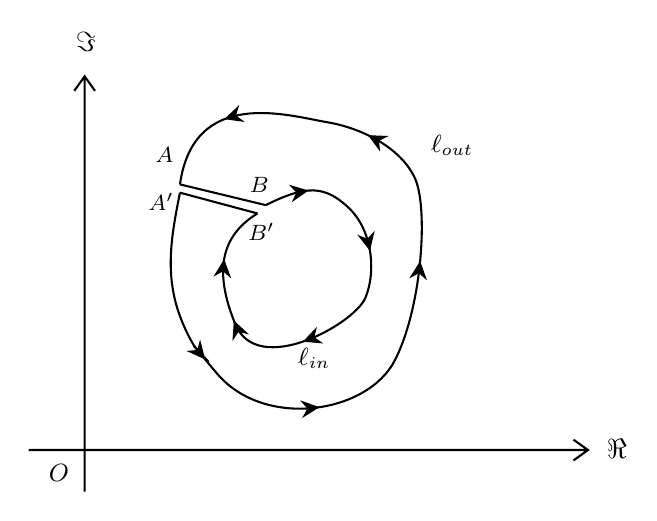
\begin{tikzpicture}[x=0.75pt,y=0.75pt,yscale=-1,xscale=1]
%uncomment if require: \path (0,300); %set diagram left start at 0, and has height of 300

%Shape: Axis 2D [id:dp04611299520330148] 
\draw  (107,219.06) -- (376.47,219.06)(133.95,39) -- (133.95,239.07) (369.47,214.06) -- (376.47,219.06) -- (369.47,224.06) (128.95,46) -- (133.95,39) -- (138.95,46)  ;
%Curve Lines [id:da4408212979573587] 
\draw    (179.87,91.07) .. controls (186.53,43.73) and (232.62,58.07) .. (250.53,61.07) .. controls (268.45,64.07) and (286.87,74.07) .. (293.2,88.4) .. controls (299.53,102.73) and (296.53,150.4) .. (283.33,175.97) .. controls (270.13,201.54) and (220.5,209.23) .. (197.65,182.12) .. controls (174.81,155.01) and (194.63,178.2) .. (193.33,175.97) ;
\draw [shift={(201.24,59.65)}, rotate = 342.17] [fill={rgb, 255:red, 0; green, 0; blue, 0 }  ][line width=0.08]  [draw opacity=0] (8.93,-4.29) -- (0,0) -- (8.93,4.29) -- (5.93,0) -- cycle    ;
\draw [shift={(270.48,67.37)}, rotate = 27.92] [fill={rgb, 255:red, 0; green, 0; blue, 0 }  ][line width=0.08]  [draw opacity=0] (8.93,-4.29) -- (0,0) -- (8.93,4.29) -- (5.93,0) -- cycle    ;
\draw [shift={(295.59,127.97)}, rotate = 96.21] [fill={rgb, 255:red, 0; green, 0; blue, 0 }  ][line width=0.08]  [draw opacity=0] (8.93,-4.29) -- (0,0) -- (8.93,4.29) -- (5.93,0) -- cycle    ;
\draw [shift={(247.14,198.42)}, rotate = 173.71] [fill={rgb, 255:red, 0; green, 0; blue, 0 }  ][line width=0.08]  [draw opacity=0] (8.93,-4.29) -- (0,0) -- (8.93,4.29) -- (5.93,0) -- cycle    ;
\draw [shift={(192.02,175.42)}, rotate = 230.07] [fill={rgb, 255:red, 0; green, 0; blue, 0 }  ][line width=0.08]  [draw opacity=0] (8.93,-4.29) -- (0,0) -- (8.93,4.29) -- (5.93,0) -- cycle    ;
%Straight Lines [id:da2752936846063838] 
\draw    (179.87,91.07) -- (221.2,101.07) ;
%Curve Lines [id:da2227786948358368] 
\draw    (221.2,101.07) .. controls (241.2,91.07) and (249.87,91.73) .. (261.2,102.4) .. controls (272.53,113.07) and (274.53,133.07) .. (269.2,145.73) .. controls (263.87,158.4) and (217.2,184.4) .. (206.53,158.4) .. controls (206.05,157.22) and (205.59,156.05) .. (205.17,154.91) .. controls (196.26,130.89) and (200.66,115.25) .. (217.2,105.07) ;
\draw [shift={(241.83,94.03)}, rotate = 170.78] [fill={rgb, 255:red, 0; green, 0; blue, 0 }  ][line width=0.08]  [draw opacity=0] (8.93,-4.29) -- (0,0) -- (8.93,4.29) -- (5.93,0) -- cycle    ;
\draw [shift={(271.41,123.08)}, rotate = 257.51] [fill={rgb, 255:red, 0; green, 0; blue, 0 }  ][line width=0.08]  [draw opacity=0] (8.93,-4.29) -- (0,0) -- (8.93,4.29) -- (5.93,0) -- cycle    ;
\draw [shift={(239.05,166.85)}, rotate = 339.24] [fill={rgb, 255:red, 0; green, 0; blue, 0 }  ][line width=0.08]  [draw opacity=0] (8.93,-4.29) -- (0,0) -- (8.93,4.29) -- (5.93,0) -- cycle    ;
\draw [shift={(205.83,156.66)}, rotate = 68.16] [fill={rgb, 255:red, 0; green, 0; blue, 0 }  ][line width=0.08]  [draw opacity=0] (8.93,-4.29) -- (0,0) -- (8.93,4.29) -- (5.93,0) -- cycle    ;
\draw [shift={(201.16,127.05)}, rotate = 95.63] [fill={rgb, 255:red, 0; green, 0; blue, 0 }  ][line width=0.08]  [draw opacity=0] (8.93,-4.29) -- (0,0) -- (8.93,4.29) -- (5.93,0) -- cycle    ;
%Straight Lines [id:da5896769090029934] 
\draw    (179.87,95.07) -- (217.2,105.07) ;
%Curve Lines [id:da07734592378285976] 
\draw    (187.2,169.73) .. controls (171.07,142.83) and (174.53,121.73) .. (179.87,95.07) ;

% Text Node
\draw (115.17,224.57) node [anchor=north west][inner sep=0.75pt]  [font=\small]  {$O$};
% Text Node
\draw (299.33,66.07) node [anchor=north west][inner sep=0.75pt]  [font=\small]  {$\ell _{out}$};
% Text Node
\draw (166.67,71.73) node [anchor=north west][inner sep=0.75pt]  [font=\footnotesize]  {$A$};
% Text Node
\draw (211.33,108.4) node [anchor=north west][inner sep=0.75pt]  [font=\footnotesize]  {$B'$};
% Text Node
\draw (212,86.4) node [anchor=north west][inner sep=0.75pt]  [font=\footnotesize]  {$B$};
% Text Node
\draw (163.33,93.73) node [anchor=north west][inner sep=0.75pt]  [font=\footnotesize]  {$A'$};
% Text Node
\draw (235.33,168.73) node [anchor=north west][inner sep=0.75pt]  [font=\small]  {$\ell _{in}$};
% Text Node
\draw (128.17,16.07) node [anchor=north west][inner sep=0.75pt]    {$\Im $};
% Text Node
\draw (384,212.4) node [anchor=north west][inner sep=0.75pt]    {$\Re $};


\end{tikzpicture}
